\chapter{Cross-Validation}
\label{ch-cross-val}

This chapter is based on Ref.\cite{wiki-xval}.

Cross-Validation (CV)
is a method 
of calculating the 
{\bf ``out-of-training-set" (OOTS) error}
for a classifier.
What this means is that the classifier 
is trained on a training set,
and its propensity to err is evaluated
on a set different from the training set.

In {\bf $k$-fold CV}, the most common CV method, 
and the only one we will discuss in this chapter,
one
partitions a  
dataset into $k$ disjoint datasets
of equal length.
One uses $k-1$ of those
sub-datasets to train a model,
and saves the last sub-dataset to
validate the model just trained.
One actually rotates which of 
the $k$ sub-datasets is used 
for validation purposes,
and calculates $k$ validation 
errors $\cale_j$ for $j=0, 1, \ldots, k-1$.
Then one averages over the $\cale_j$
to obtain a final OOTS error $\cale$. 

CV strongly resembles
Jackknife
Resampling (JR) 
(see Chapter \ref{ch-jack}),
but in JR 
the validation sub-dataset is
never used for anything,
whereas in CV,
it is used for validation
purposes, to calculate
an OOTS error.

Next, we will
explain $k$-fold CV more explicitly,
using 
equations and a bnet.


Let $L=[0,1,2, \ldots, nsam-1]$ be a list of
individuals (samples) in a population.
In this chapter, we will use the notation 
$A^\s=A[\s]$ 
and $\vec{A}=[A^\s:\s\in L]$
for a  list (vector, 1-D  array) indexed by $L$.
We will refer to $DS=(\vec{x}, \vec{y})$ 
where $x^\s\in S_\rvx$, $y^\s\in S_\rvy$,
as a dataset.
If
$L_j$ is a list (possibly with 
duplicate items)
such that $set(L_j)\subset set(L)$, then
define
$DS_j=(\vec{x}, \vec{y})_{L_j}=
((x^\s)_{\s\in L_j}, 
(y^\s)_{\s\in L_j})$.
We will
refer to $DS_j$
as the {\bf restriction of 
$(\vec{x}, \vec{y})$ to $L_j$.}

Let
$J=\{0,1, 2, \ldots, nj-1\}$.

Define a {\bf training list(TL),
validation list(VL) pair} $(TL,VL)$
to be a pair of lists
such that 
$set(TL)$ and $set(VL)$
are disjoint subsets
of $set(L)$.
Let $(TL_j, VL_j)$ for $j\in J$
be $nj$ such TL-VL pairs.


Fig.\ref{fig-xfold-xval} 
shows
the TL-VL pairs 
that are used
when doing $k$-fold 
CV.
In that figure, $k=nj=4$.
As you can see,
in $k$-fold CV, one chooses 
$nj=k$ list pairs $(TL_j, VL_j)$
such that all individuals $\s\in L$
appear exactly once, in either
$TL_j$ or $TV_j$, but not in both.

\begin{figure}[h!]
\centering
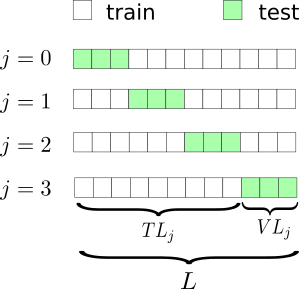
\includegraphics[width=2in]
{cross-val/kfold-xval.png}
\caption{4-fold CV with $|L|=12$.
For all $j$,
$|VL_j|=3$ and $|TL_j|=9$. 
All individuals $\s\in L$
appear exactly once, in either
$TL_j$ or $TV_j$, but not in both.} 
\label{fig-xfold-xval}
\end{figure}

We will refer to a function
$Y:S_\rvx \rarrow S_\rvc$ as a
classifier. It maps a vector
of features $x$
to a class $c$. 
Let
$Y_j$ for $j\in J$
denote $nj$ classifiers.


If $Y_j:S_\rvx\rarrow S_\rvc$
and $S_\rvc$ is a discrete
set (``categorical"),
then define the {\bf OOTS error
for the $j$th classifier} as:
 
\begin{subequations}
\label{eq-err-j-def}
\beq
\cale_j=
\frac{1}{|VL_j|}
\sum_{\s\in VL_j}
\indi(y^\s\neq Y_j(x^\s))
\;.
\eeq
On the other hand,
if $S_\rvc=\RR$,
it makes more sense to
define $\cale_j$
as a mean square error:

\beq
\cale_j=
\frac{1}{|VL_j|}
\sum_{\s\in VL_j}
(y^\s-Y_j(x^\s))^2
\;.
\eeq
\end{subequations}
Finally,
define the {\bf final OOTS} error as

\beq
\cale=
\frac{1}{|J|}\sum_{j\in J} \cale_j
\;.
\label{eq-fin-err-def}
\eeq

Fig.\ref{fig-bnet-CV}
gives a bnet 
that represents
the CV algorithm.
The TPMs, printed  in blue, for the
bnet Fig.\ref{fig-bnet-CV},
are as follows:

\begin{figure}
$$
\xymatrix{
&&(\vec{\rvx}, \vec{\rvy})
\ar[d]\ar[dr]\ar[drr]\ar[drrr]
\ar[dl]\ar[dll]
\\
(\vec{\rvx}, \vec{\rvy})_{TL_0}\ar[d]
&
(\vec{\rvx}, \vec{\rvy})_{VL_0}\ar[ldd]
&
(\vec{\rvx}, \vec{\rvy})_{TL_1}\ar[d]
&
(\vec{\rvx}, \vec{\rvy})_{VL_1}\ar[ldd]
&
(\vec{\rvx}, \vec{\rvy})_{TL_2}\ar[d]
&
(\vec{\rvx}, \vec{\rvy})_{VL_2}\ar[ldd]
\\
\rvY_0\ar[d]
&&\rvY_1\ar[d]
&&\rvY_2\ar[d]
\\
\ul{\cale}_0\ar[drr]
&&\ul{\cale}_1\ar[d]
&&\ul{\cale}_2\ar[dll]
\\
&&\ul{\cale}
}
$$
\caption{
Bnet for 3-fold CV.}
\label{fig-bnet-CV}
\end{figure}

\beq\color{blue}
P((\vec{x}, \vec{y})_{TL_j}|
(\vec{x}, \vec{y}))=
\indi(\;\;\;(\vec{x},\vec{y})_{TL_j} =
\text{restriction of
$(\vec{x}, \vec{y})$ to
$TL_j$.}\;\;\; )
\eeq

\beq\color{blue}
P((\vec{x}, \vec{y})_{VL_j}|
(\vec{x}, \vec{y}))=
\indi(\;\;\;(\vec{x}, \vec{y})_{VL_j}=
\text{restriction of
$(\vec{x}, \vec{y})$
to $VL_j$.}\;\;\; )
\eeq
  
\beq\color{blue}
P(Y_j|(\vec{x},\vec{y})_{TL_j})
=
\indi(\;\;\;
Y_j= \text{classifier
trained with 
$(\vec{x},\vec{y})_{TL_j}$}
\;\;\;)
\eeq

\beq\color{blue}
P(\cale_j|Y_j, 
(\vec{x},\vec{y})_{VL_j})
=
\indi(\;\;\;
\cale_j=
\text{ defined by Eqs.(\ref{eq-err-j-def}).}
\;\;\;)
\eeq


\beq\color{blue}
P(\cale|(\cale_j)_{j\in J})=
\indi(
\;\;\;
\cale=\text{ defined by Eq.(\ref{eq-fin-err-def}).}
\;\;\;)
\eeq